\documentclass[xcolor={table}]{beamer}
\usetheme{Singapore}
\usepackage[utf8]{inputenc}
\usecolortheme{crane}
\usepackage{graphicx}
\usepackage{iwona}
\usepackage{standalone}
\usepackage{tikz}
\usetikzlibrary{arrows}
\usetikzlibrary{decorations.markings}
\usetikzlibrary{calc}
\usetikzlibrary{shapes,snakes}
\usepackage{amsmath}
\usepackage{amsfonts}
\usepackage{amsthm}
\usepackage{mathtools}

\definecolor{lightblue}{RGB}{124,190,255}
\definecolor{darkgreen}{RGB}{24,145,0}

\beamertemplatenavigationsymbolsempty
\setbeamerfont{caption}{size=\tiny}


\title
{Queueing Networks for a Healthcare System}
\subtitle
{Deadlocking \& Reinforcement Learning}
\author{Geraint Palmer\newline \scriptsize{Paul Harper, Vincent Knight}}
\date{Young OR 19 - Aston University 2015}
\titlegraphic{
\includegraphics[width=1.5cm]{cflogo}}

\begin{document}
\frame{\titlepage}

% THE PROBLEM - HEALTH BOARD, WORKFORCE PLANNING ETC

% 1st slide, health_system map
\begin{frame}
\frametitle{Aneurin Bevan University Health Board}
\begin{figure}
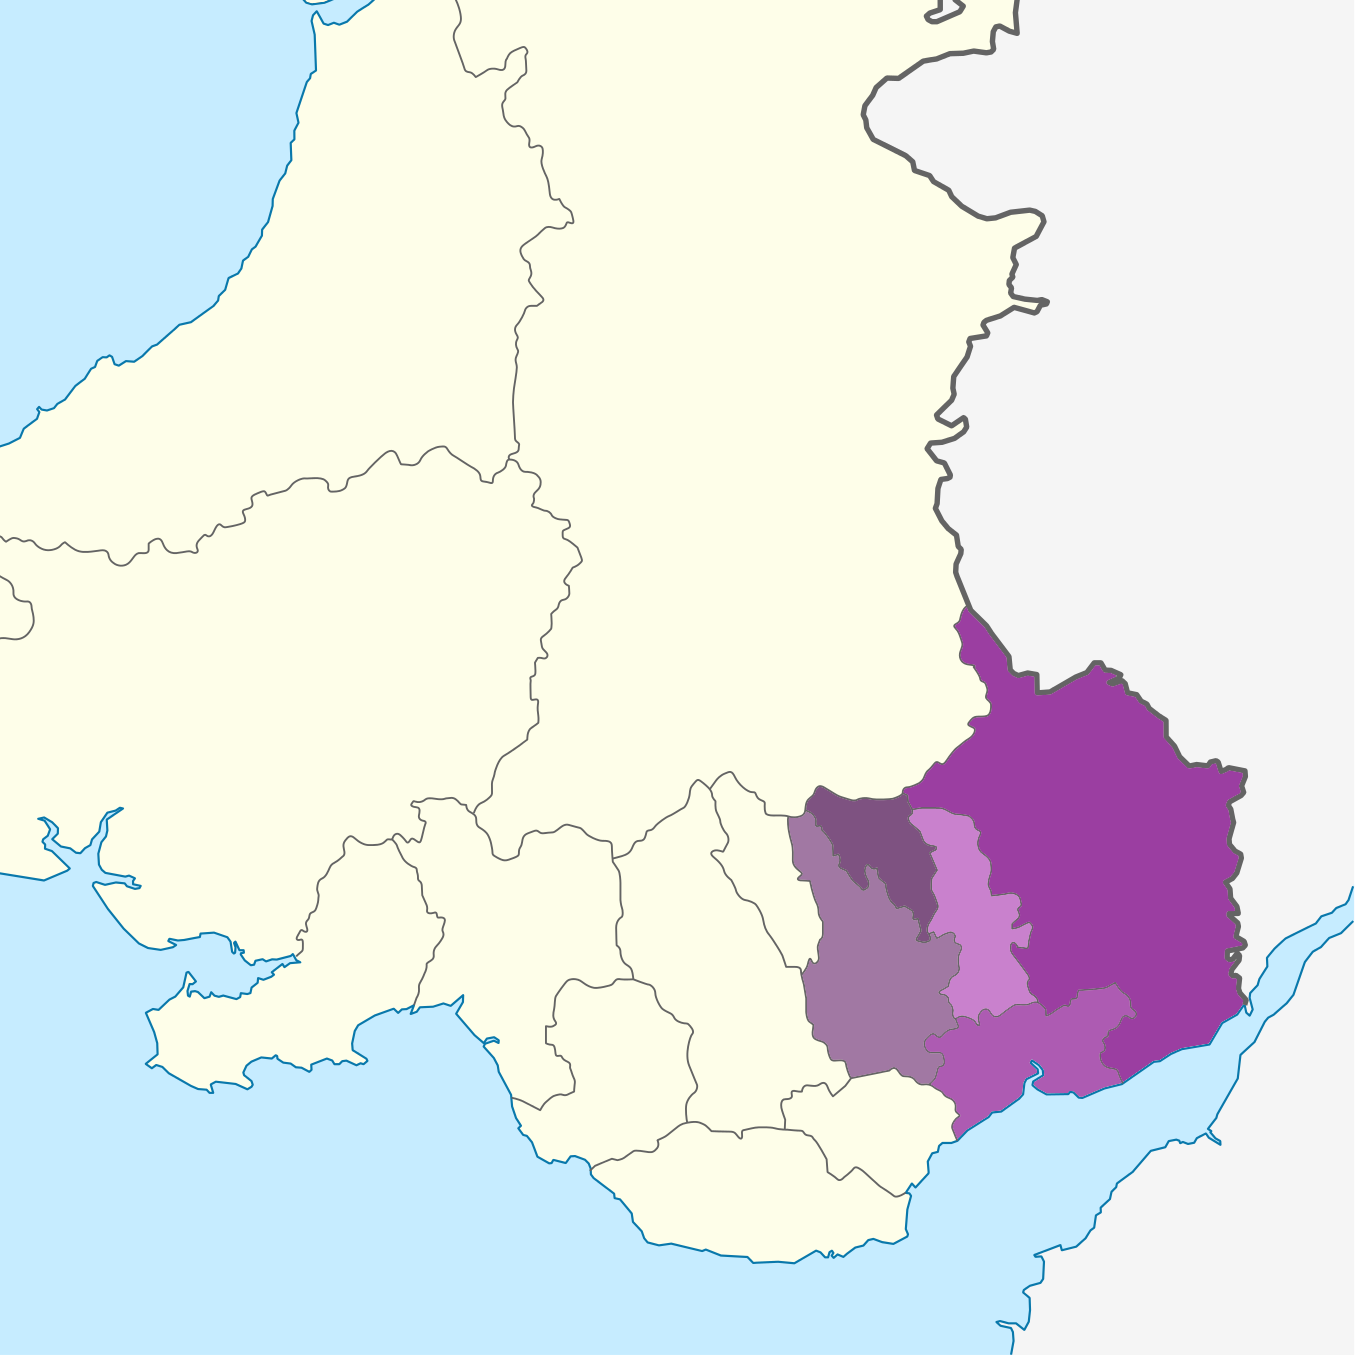
\includegraphics[width=0.7\textwidth]{Aneurin_Bevan}
\end{figure}
\end{frame}


% % 3rd slide, example final product
% \begin{frame}
%     \includestandalone[width=\textwidth]{end_product}
% \end{frame}

% % 3rd slide, example final product
% \begin{frame}
%     \includestandalone[width=\textwidth]{end_product_results}
% \end{frame}


% 1st slide, health_system map
\begin{frame}
\frametitle{Map of Healthcare System}
\begin{figure}
\includestandalone[width=\textwidth]{health_system}
\end{figure}
\end{frame}

% QUEUEING NETWORKS

% Unrestricted
\begin{frame}
  \frametitle{Jackson Networks}
  \begin{figure}
  \includestandalone[width=\textwidth]{jacksonnet}
  \end{figure}
\end{frame}
\begin{frame}
  \frametitle{Jackson Networks}
  \begin{figure}
  \includestandalone[width=\textwidth]{jacksonnet3}
  \end{figure}
\end{frame}

% Resticted
\begin{frame}
  \frametitle{Restricted Networks}
  \begin{figure}
  \includestandalone[width=\textwidth]{restrictnet}
  \end{figure}
\end{frame}

\begin{frame}
  \frametitle{Restricted Networks}
  \begin{itemize}
    \item Markov Chain Models
    \item Approximation Methods
    \item Simulation
  \end{itemize}
\end{frame}


% DEADLOCK

\begin{frame}
    \frametitle{Deadlock}
    \begin{figure}
    \includestandalone[width=0.7\textwidth]{gridlock}
    \end{figure}
\end{frame}

\begin{frame}
    \begin{figure}
    \includestandalone[width=\textwidth]{buildupdigraph}
    \end{figure}
\end{frame}

% Types of Deadlock
\begin{frame}
    \frametitle{Types of Deadlock}
    \begin{columns}
        \column{0.5\textwidth}
        \center
        Transient Deadlock
        \begin{figure}
        \includestandalone[width=\textwidth]{transientdeadlock}
        \end{figure}
        \column{0.5\textwidth}
        \center
        Absorbing Deadlock
        \begin{figure}
        \includestandalone[width=\textwidth]{absorbingdeadlock}
        \end{figure}
    \end{columns}
\end{frame}

\begin{frame}
    \frametitle{Deadlock Configurations}
    \begin{columns}
        \column{0.5\textwidth}
        \center
        Transient Deadlock
        \begin{figure}
        \includestandalone[width=\textwidth]{transientdeadlockconfigs}
        \end{figure}
        \column{0.5\textwidth}
        \center
        Absorbing Deadlock
        \begin{figure}
        \includestandalone[width=\textwidth]{absorbingdeadlockconfigs}
        \end{figure}
    \end{columns}
\end{frame}


% Markovian deadlock model 1 Node
\begin{frame}
    \frametitle{Markovian Model of Deadlock}
    \includestandalone[width=\textwidth]{1nodeexample}\newline
    \center{\LARGE{$(i)$}}
\end{frame}


\begin{frame}
%\frametitle{Markovian Model of Deadlock}
\center
\scriptsize \[S = \{i\in\mathbb{N}| 0 \leq i \leq n + 1\}\cup\{-1\}\]
Define $\delta = i_2 - i_1$\newline

\vspace{6 mm}

  $q_{i_1, i_2} = \left\{
  \begin{matrix*}[ r ]
    \left. \color{red} \begin{matrix*}[ r ]
      \Lambda & \text{if } i < n + 1 \\
      0 & \text{otherwise}
    \end{matrix*} \right\} & \color{red} \text{if } \delta = 1 \\
    \color{blue} (1 - r_{11})\mu & \color{blue} \text{if } \delta = -1 \\
    \color{blue} 0 & \color{blue} \text{otherwise}
  \end{matrix*} \right.$
\vspace{6 mm}

$q_{i, -1} = \left\{ \color{darkgreen}
  \begin{matrix*}[ r ]
    r_{11}\mu & \text{if } i = n + 1 \\
    0 & \text{otherwise}
  \end{matrix*}
  \right.$

\vspace{6 mm}

$q_{-1, s} = 0$
\end{frame}

\begin{frame}
    \begin{figure}
    \includestandalone[width=0.95\textwidth]{markov_chain_1node}
    \end{figure}
\end{frame}

\begin{frame}
    \frametitle{Times to Deadlock}
    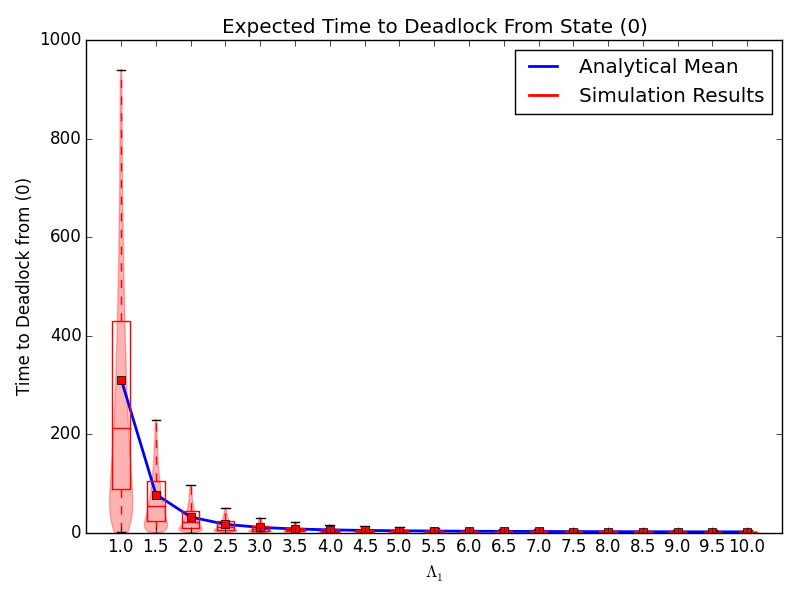
\includegraphics[width=0.5\textwidth]{varyL1_1node}
    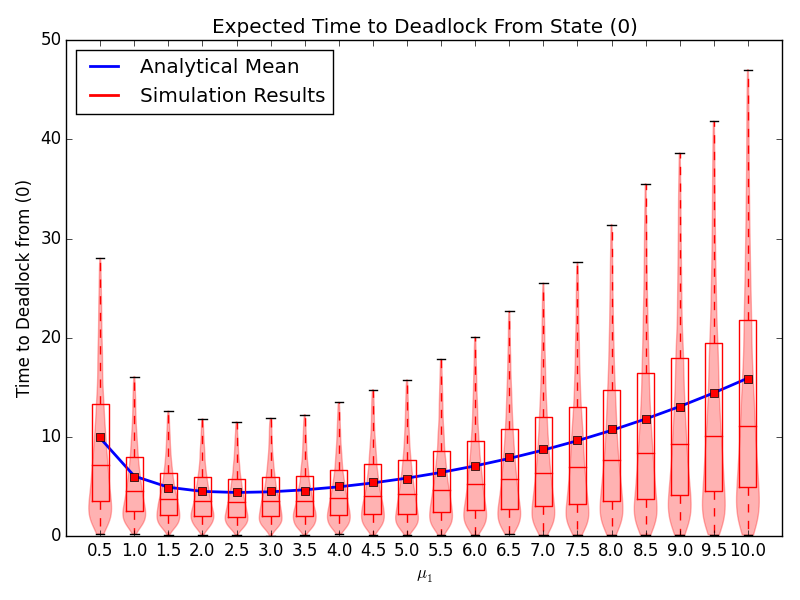
\includegraphics[width=0.5\textwidth]{varymu1_1node}\newline
    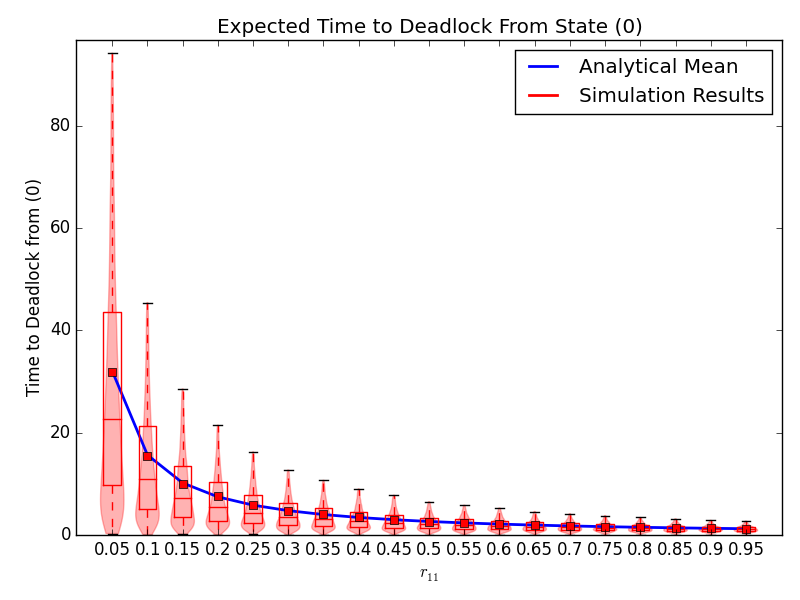
\includegraphics[width=0.5\textwidth]{varyr11_1node}
    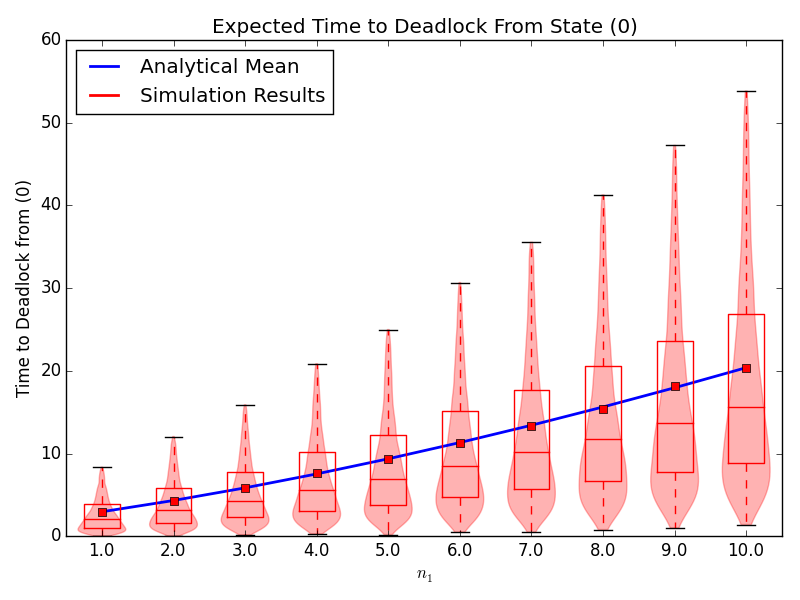
\includegraphics[width=0.5\textwidth]{varyn1_1node}
\end{frame}



% Markov deadlock model 2 Node
\begin{frame}
    \frametitle{Markovian Model of Deadlock}
    \includestandalone[width=\textwidth]{2nodeexample}\newline
    \center{\LARGE{$(i, j)$}}
\end{frame}


\begin{frame}
%\frametitle{Markovian Model of Deadlock}
\center
\scriptsize \[S = \{(i,j)\in\mathbb{N}^{(n_1+2\times n_2+2)}| 0 \leq i + j \leq n_1 + n_2 + 2\}\cup\{(-1)\}\]
Define $\delta = (i_2, j_2) - (i_1, j_1)$\newline

  $q_{(i_1, j_1),(i_2, j_2)} = \left\{
  \begin{matrix*}[ r ]
    \left. \color{red} \begin{matrix*}[ r ]
      \Lambda_1 & \text{if } i_1 \leq n_1 \\
      0 & \text{otherwise}
    \end{matrix*} \right\} & \color{red} \text{if } \delta = (1, 0)\\
    \left. \color{orange} \begin{matrix*}[ r ]
      \Lambda_2 & \text{if } j_1 \leq n_2 \\
      0 & \text{otherwise}
    \end{matrix*} \right\} & \color{orange} \text{if } \delta = (0, 1) \\
    \left. \color{blue} \begin{matrix*}[ r ]
      (1 - r_{12})\mu_1 & \color{blue} \text{if } j_1 < n_2 + 2 \\
      0 & \text{otherwise}
    \end{matrix*} \right\} & \color{blue} \text{if } \delta = (-1, 0) \\
    \left. \color{lightblue} \begin{matrix*}[ r ]
      (1 - r_{21})\mu_2 & \text{if } i_1 < n_1 + 2 \\
      0 & \color{lightblue} \text{otherwise}
    \end{matrix*} \right\} & \color{lightblue} \text{if } \delta = (0, -1) \\
    \left. \color{darkgreen} \begin{matrix*}[ r ]
      r_{12}\mu_1 & \text{if } j_1 < n_2 + 2 \text{ and } (i_1, j_1) \neq (n_1+2, n_2) \\
      0 & \text{otherwise}
    \end{matrix*} \right\} & \color{darkgreen} \text{if } \delta = (-1, 1) \\
    \left. \color{green} \begin{matrix*}[ r ]
      r_{21}\mu_2 & \text{if } i_1 < n_1 + 2 \text{ and } (i_1, j_1) \neq (n_1, n_2+2)\\
      0 & \text{otherwise}
    \end{matrix*} \right\} & \color{green} \text{if } \delta = (1, -1) \\
    0 & \text{otherwise}
  \end{matrix*} \right.$\newline\newline

$q_{(i_1, j_1), (-1)} = \left\{
  \begin{matrix*}[ r ]
    \color{green} r_{21}\mu_2 & \color{green} \text{if } (i, j) = (n_1, n_2 + 2) \\
    \color{darkgreen} r_{12}\mu_1 & \color{darkgreen} \text{if } (i, j) = (n_1 + 2, n_2) \\
    0 & \text{otherwise}
  \end{matrix*}
  \right.$\newline\newline
$q_{-1, s} = 0$
\end{frame}

\begin{frame}
    \begin{figure}
    \includestandalone[width=0.95\textwidth]{markov_chain}
    \end{figure}
\end{frame}

\begin{frame}
    \frametitle{Times to Deadlock}
    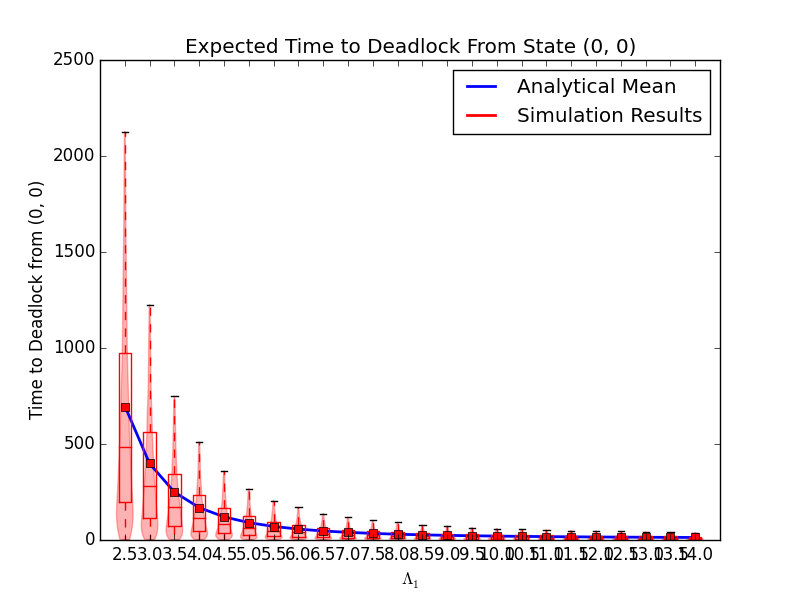
\includegraphics[width=0.5\textwidth]{varyL1}
    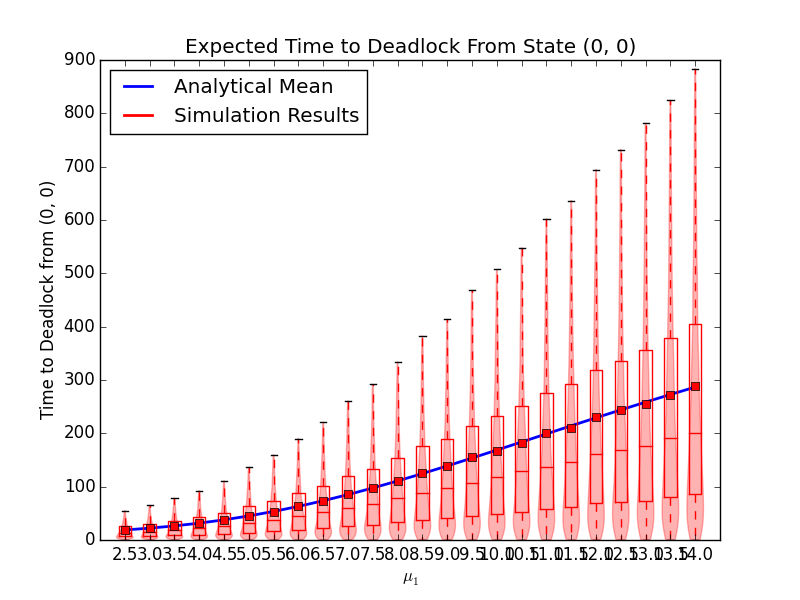
\includegraphics[width=0.5\textwidth]{varymu1}\newline
    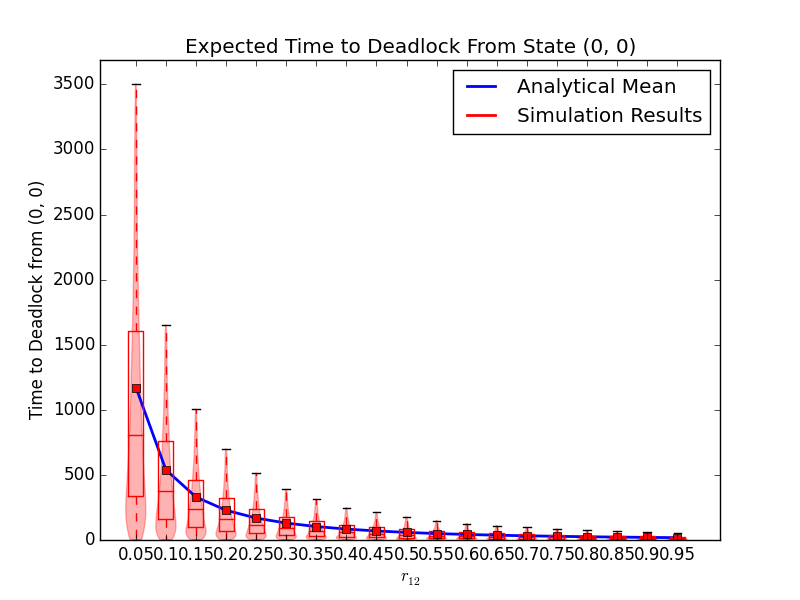
\includegraphics[width=0.5\textwidth]{varyr12}
    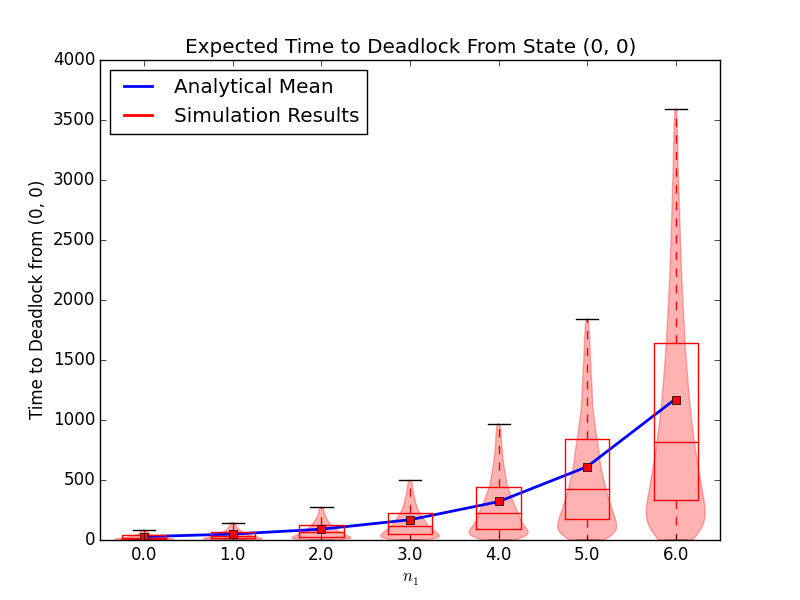
\includegraphics[width=0.5\textwidth]{varyn1}
\end{frame}


% Markov deadlock model 2 Node self loops
\begin{frame}
    \frametitle{Markovian Model of Deadlock}
    \includestandalone[width=\textwidth]{2nodefeedbackexample}\newline
    \center{\LARGE{$(i, j)$}}
\end{frame}


\begin{frame}
%\frametitle{Markovian Model of Deadlock}
\center
\scriptsize \[S = \{(i,j)\in\mathbb{N}^{(n_1+2\times n_2+2)}| 0 \leq i + j \leq n_1 + n_2 + 2\}\cup\{(-1)\}\]
Define $\delta = (i_2, j_2) - (i_1, j_1)$\newline\newline
\tiny{
  $q_{(i_1, j_1),(i_2, j_2)} = \left\{
  \begin{matrix*}[ r ]
    \left. \color{red} \begin{matrix*}[ r ]
      \Lambda_1 & \text{if } i_1 \leq n_1 \\
      0 & \text{otherwise}
    \end{matrix*} \right\} & \color{red} \text{if } \delta = (1, 0)\\
    \left. \color{orange} \begin{matrix*}[ r ]
      \Lambda_2 & \text{if } j_1 \leq n_2 \\
      0 & \text{otherwise}
    \end{matrix*} \right\} & \color{orange} \text{if } \delta = (0, 1) \\
    \left. \color{blue} \begin{matrix*}[ r ]
      (1 - r_{12})\mu_1 & \color{blue} \text{if } j_1 < n_2 + 2 \\
      0 & \text{otherwise}
    \end{matrix*} \right\} & \color{blue} \text{if } \delta = (-1, 0) \\
    \left. \color{lightblue} \begin{matrix*}[ r ]
      (1 - r_{21})\mu_2 & \text{if } i_1 < n_1 + 2 \\
      0 & \color{lightblue} \text{otherwise}
    \end{matrix*} \right\} & \color{lightblue} \text{if } \delta = (0, -1) \\
    \left. \color{darkgreen} \begin{matrix*}[ r ]
      r_{12}\mu_1 & \text{if } j_1 < n_2 + 2 \text{ and } (i_1, j_1) \neq (n_1+2, n_2) \\
      0 & \text{otherwise}
    \end{matrix*} \right\} & \color{darkgreen} \text{if } \delta = (-1, 1) \\
    \left. \color{green} \begin{matrix*}[ r ]
      r_{21}\mu_2 & \text{if } i_1 < n_1 + 2 \text{ and } (i_1, j_1) \neq (n_1, n_2+2)\\
      0 & \text{otherwise}
    \end{matrix*} \right\} & \color{green} \text{if } \delta = (1, -1) \\
    0 & \text{otherwise}
  \end{matrix*} \right.$\newline\newline

  $q_{(i_1, j_1), (-1)} = \left\{
  \begin{matrix*}[ r ]
    \color{magenta!50} r_{11}\mu_1 & \color{magenta!50} \text{if } i > n_1 \text{ and } j < n_2 + 2 \\
    0 & \text{otherwise}
  \end{matrix*}
  \right.$\newline

  $q_{(i_1, j_1), (-2)} = \left\{
  \begin{matrix*}[ r ]
    \color{violet!50} r_{22}\mu_2 & \color{violet!50} \text{if } j > n_2 \text{ and } i < n_1 + 2 \\
    0 & \text{otherwise}
  \end{matrix*}
  \right.$\newline

  $q_{(i_1, j_1), (-3)} = \left\{
  \begin{matrix*}[ r ]
    \color{green} r_{21}\mu_2 & \color{green} \text{if } (i, j) = (n_1, n_2 + 2) \\
    \color{darkgreen} r_{12}\mu_1 & \color{darkgreen} \text{if } (i, j) = (n_1 + 2, n_2) \\
    0 & \text{otherwise}
  \end{matrix*}
  \right.$\newline

$q_{-1, s} = q_{-2, s} = q_{-3, s} = 0$
}
\end{frame}

\begin{frame}
    \begin{figure}
    \includestandalone[width=0.95\textwidth]{markov_chain_feedback}
    \end{figure}
\end{frame}

\begin{frame}
    \frametitle{Times to Deadlock}
    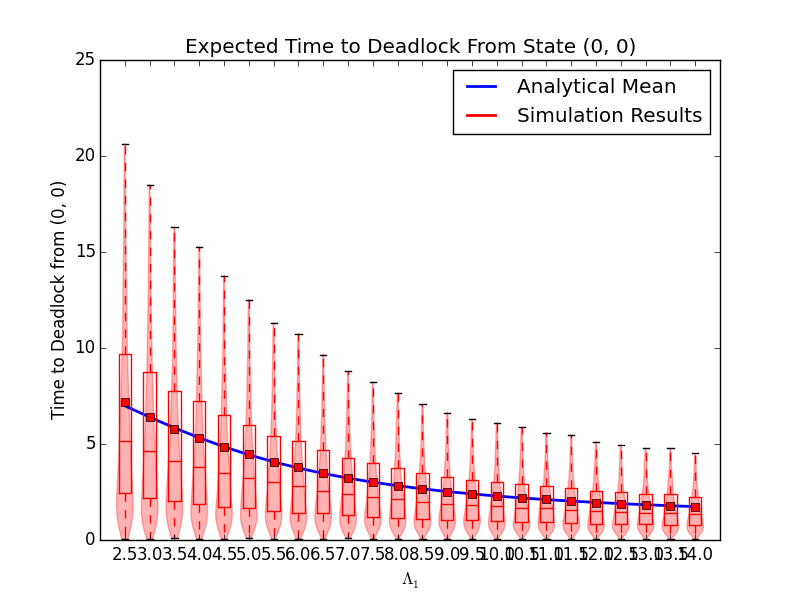
\includegraphics[width=0.5\textwidth]{vary_L1fb}
    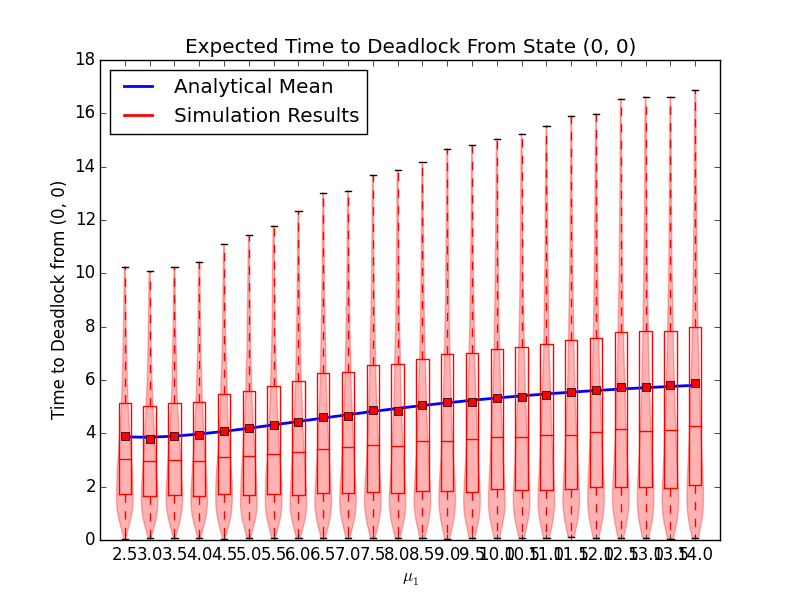
\includegraphics[width=0.5\textwidth]{vary_mu1fb}\newline
    \centering
    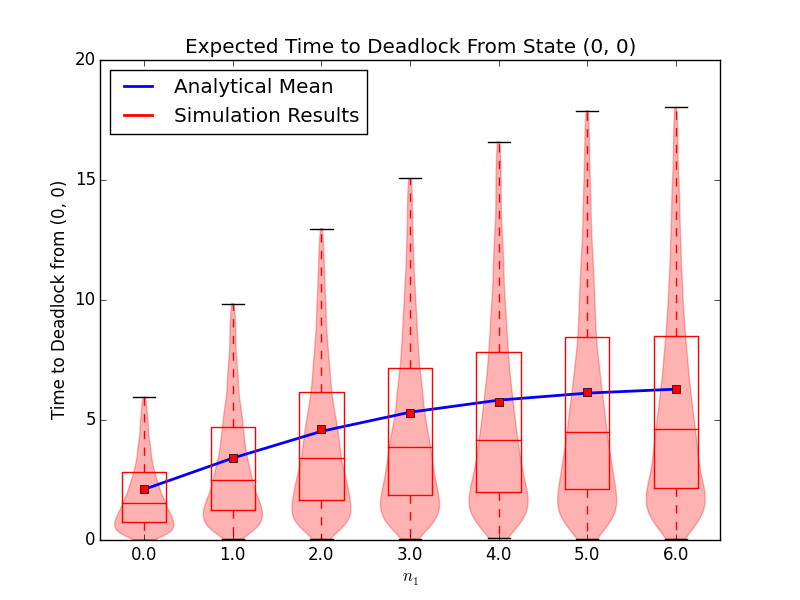
\includegraphics[width=0.5\textwidth]{vary_n1fb}
\end{frame}


% REINFORCEMENT LEARNING

\begin{frame}
    \frametitle{Reinforcement Learning}
    \only<1>{
    \begin{figure}
    \includestandalone[width=\textwidth]{health_system}
    \end{figure}
    }
    \only<2>{
    \begin{figure}
    \includestandalone[width=0.8\textwidth]{qlearn_flowchart}
    \end{figure}
    }
    \only<3>{
    Q-Learning
    \begin{equation*}
    Q(s, a) \leftarrow Q(s, a) + \alpha [ r + \gamma \text{max}_{a'} Q(s', a') - Q(s, a)]
    \end{equation*}
    }
\end{frame}

\begin{frame}
  \frametitle{Reinforcement Learning}

  \begin{table}

  \begin{tabular}{ | c | c | c | c | }
  \hline
  $s_n$ & $a_1$ & $a_2$ & $a_3$ \\
  \hline
  $n = 0$ & \cellcolor{green} $10.2$ & $3.3$ & $-2.1$ \\
  $n = 1$ & \cellcolor{green} $9.4$ & $2.1$ & $-0.7$ \\
  $n = 2$ & \cellcolor{green} $9.5$ & $3.8$ & $1.6$ \\
  $n = 3$ & \cellcolor{green} $8.3$ & $5.4$ & $5.3$ \\
  $n = 4$ & $3.1$ & \cellcolor{green} $9.2$ & $6.7$ \\
  $n = 5$ & $4.0$ & $6.1$ & \cellcolor{green} $6.7$ \\
  $n = 6$ & $0.2$ & $6.3$ & \cellcolor{green} $7.5$ \\
  \hline
  \end{tabular}
  \caption{Example table of $Q(s, a)$}
  \end{table}
\end{frame}

\begin{frame}
    \frametitle{Diolch - Thank You}
    https://github.com/geraintpalmer/Presentations
    palmergi1@cardiff.ac.uk
\end{frame}

\end{document}
